\documentclass[12pt,letterpaper]{article}

\usepackage{amsmath, amsthm}
\usepackage{microtype, parskip}
\usepackage[comma,numbers,sort&compress]{natbib}
\usepackage{lineno}
\usepackage{docmute}
\usepackage{caption, subcaption, multirow, morefloats, rotating}
\usepackage{wrapfig}

\frenchspacing

\begin{document}

\section*{Results}

\subsection*{Comparing the fits of the pure-presence and birth-death models}

\begin{figure}[ht]
  \centering
  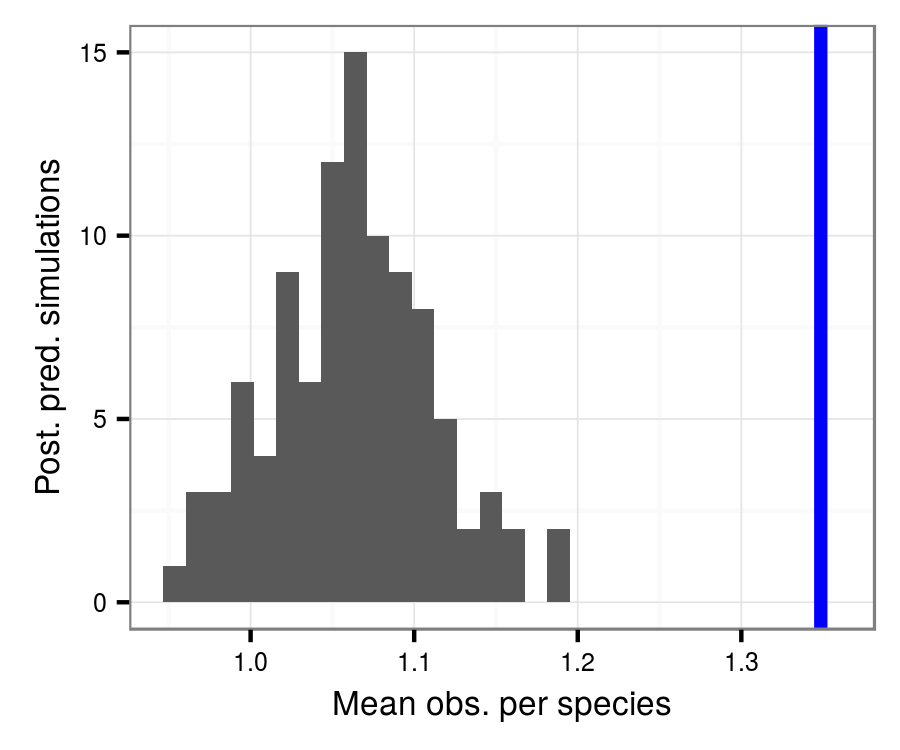
\includegraphics[width=\textwidth,height=0.4\textheight,keepaspectratio=true]{figure/pred_occ}
  \caption{Posterior predictive check for pure-presence model.}
  \label{fig:ppc_pure_presence}
\end{figure}

\begin{figure}[ht]
  \centering
  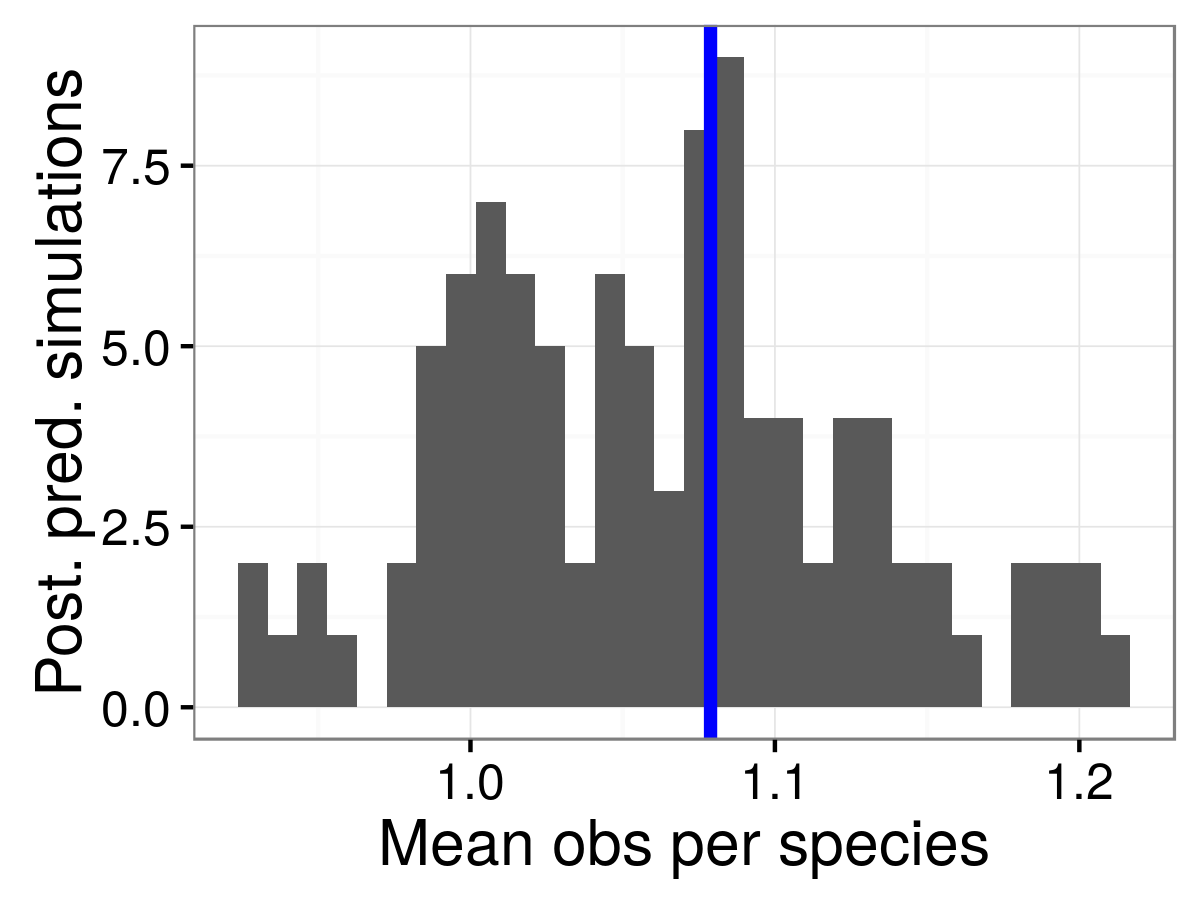
\includegraphics[width=\textwidth,height=0.4\textheight,keepaspectratio=true]{figure/pred_occ_bd}
  \caption{Posterior predictive check for birth-death model.}
  \label{fig:ppc_birth_death}
\end{figure}

\begin{figure}[ht]
  \centering
  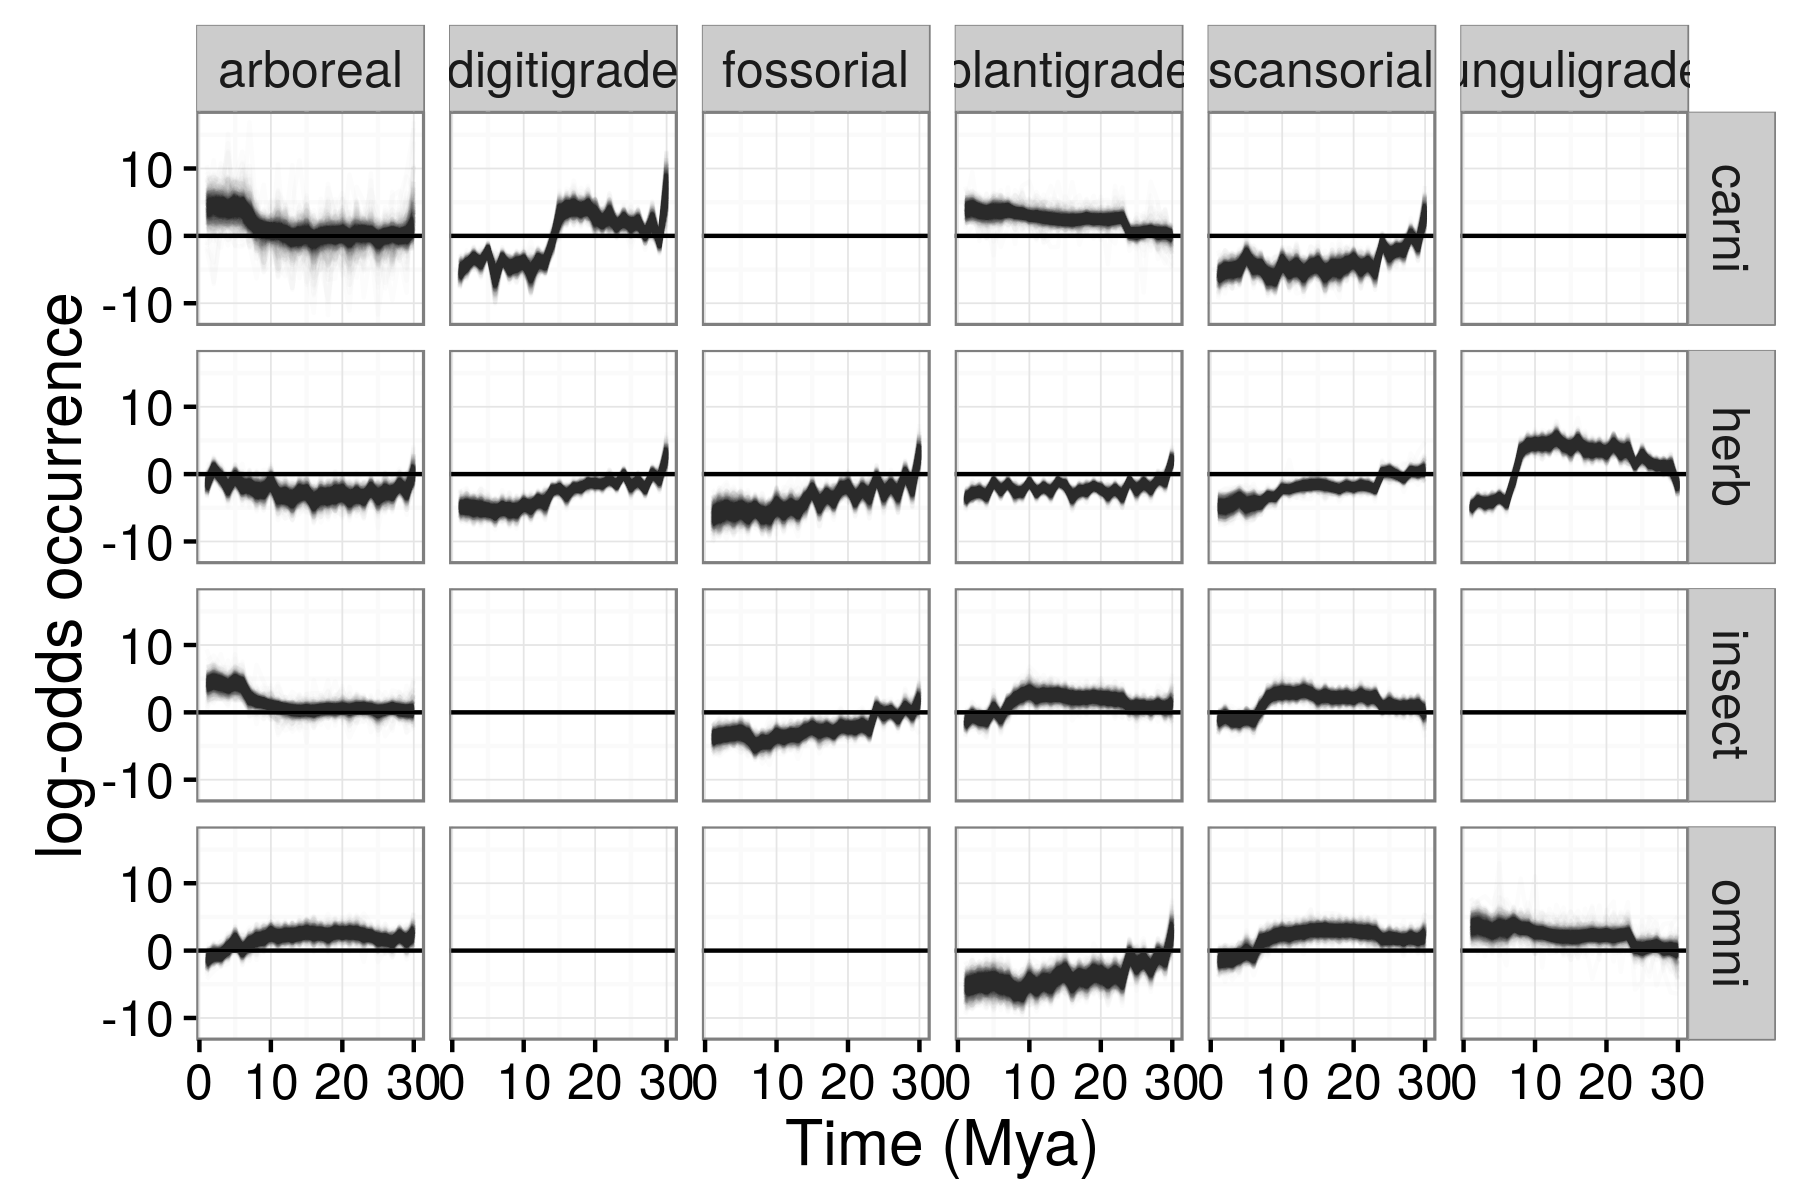
\includegraphics[width=\textwidth,height=0.8\textheight,keepaspectratio=true]{figure/ecotype_occurrence}
  \caption{Probability of ecotype occurring over time. Estimates are from the pure-presence model.}
  \label{fig:eco_occur}
\end{figure}

\begin{figure}[ht]
  \centering
  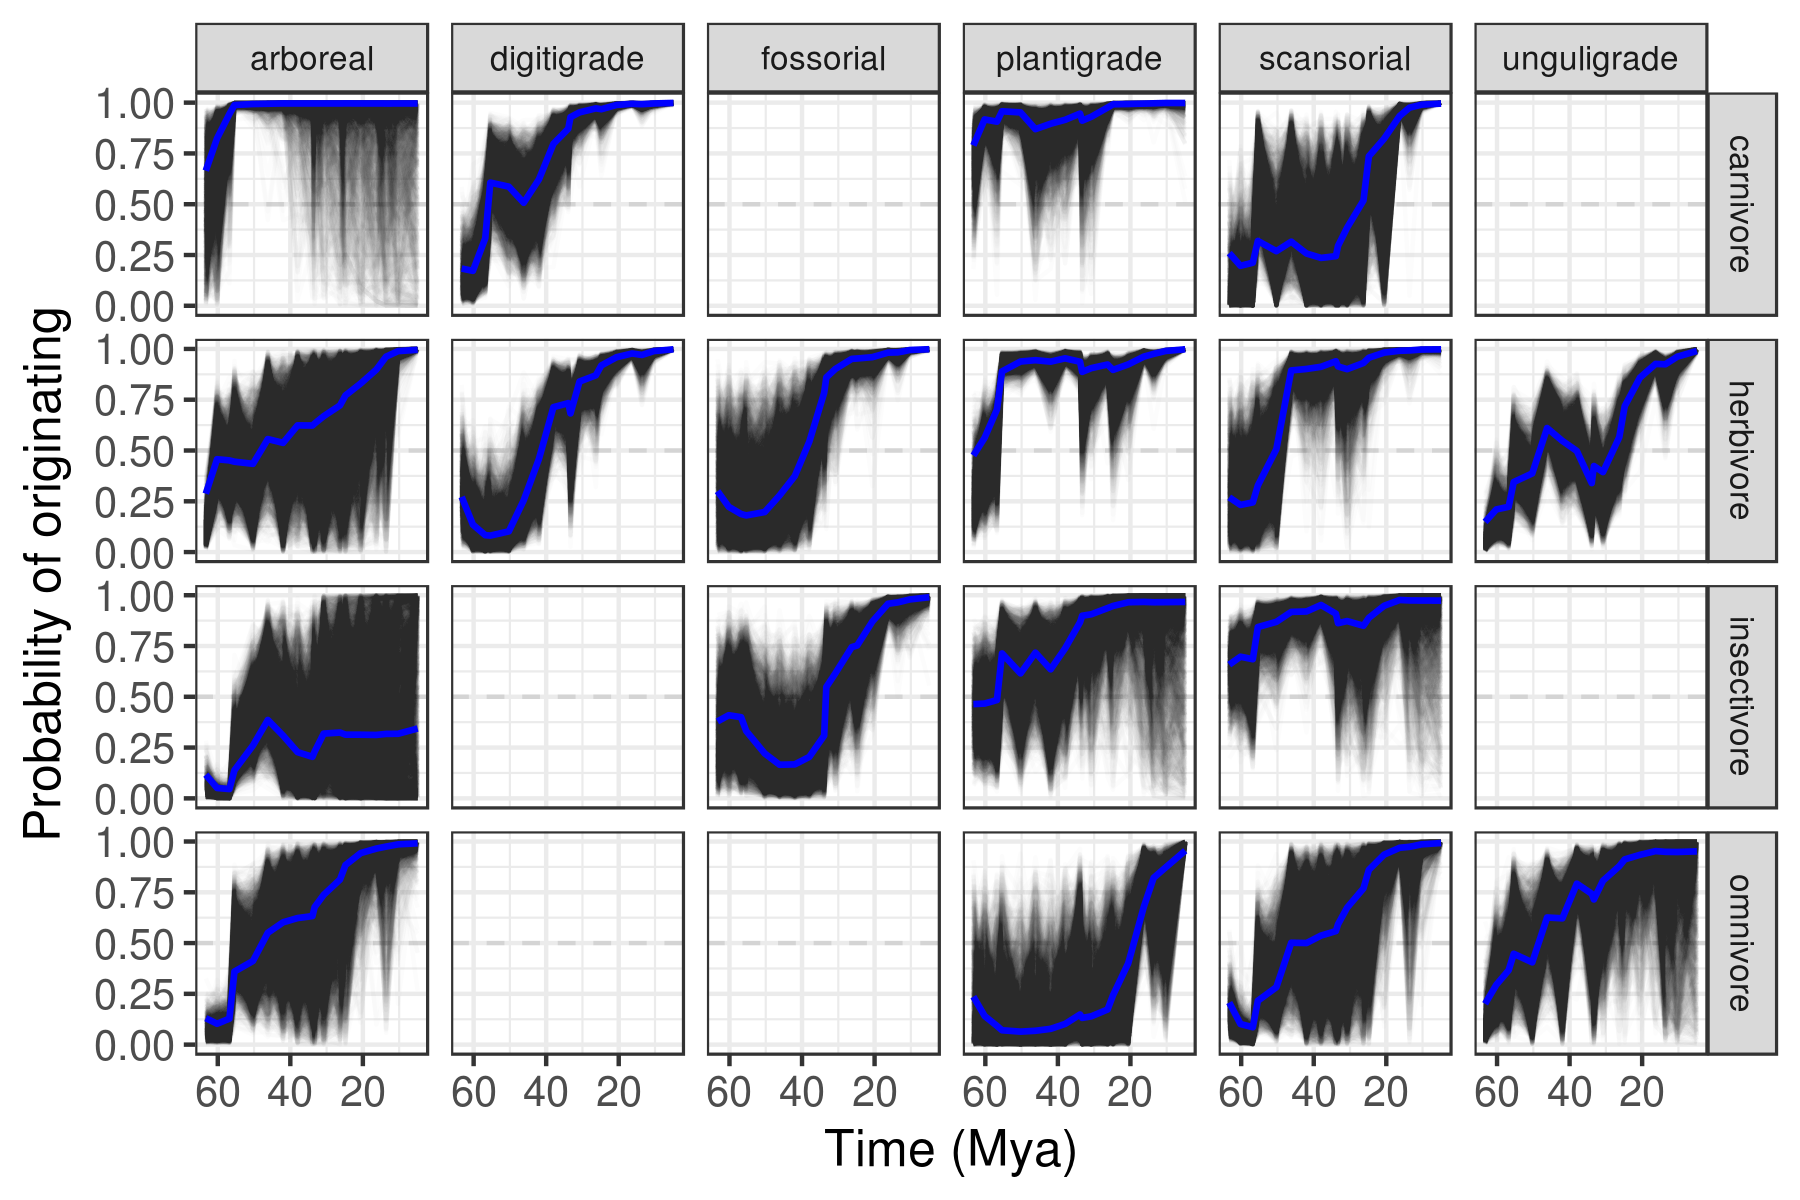
\includegraphics[width=\textwidth,height=0.8\textheight,keepaspectratio=true]{figure/ecotype_origin_bd}
  \caption{Probability of species origination by ecotype. Estimates are from the birth-death model.}
  \label{fig:eco_origin}
\end{figure}

\begin{figure}[ht]
  \centering
  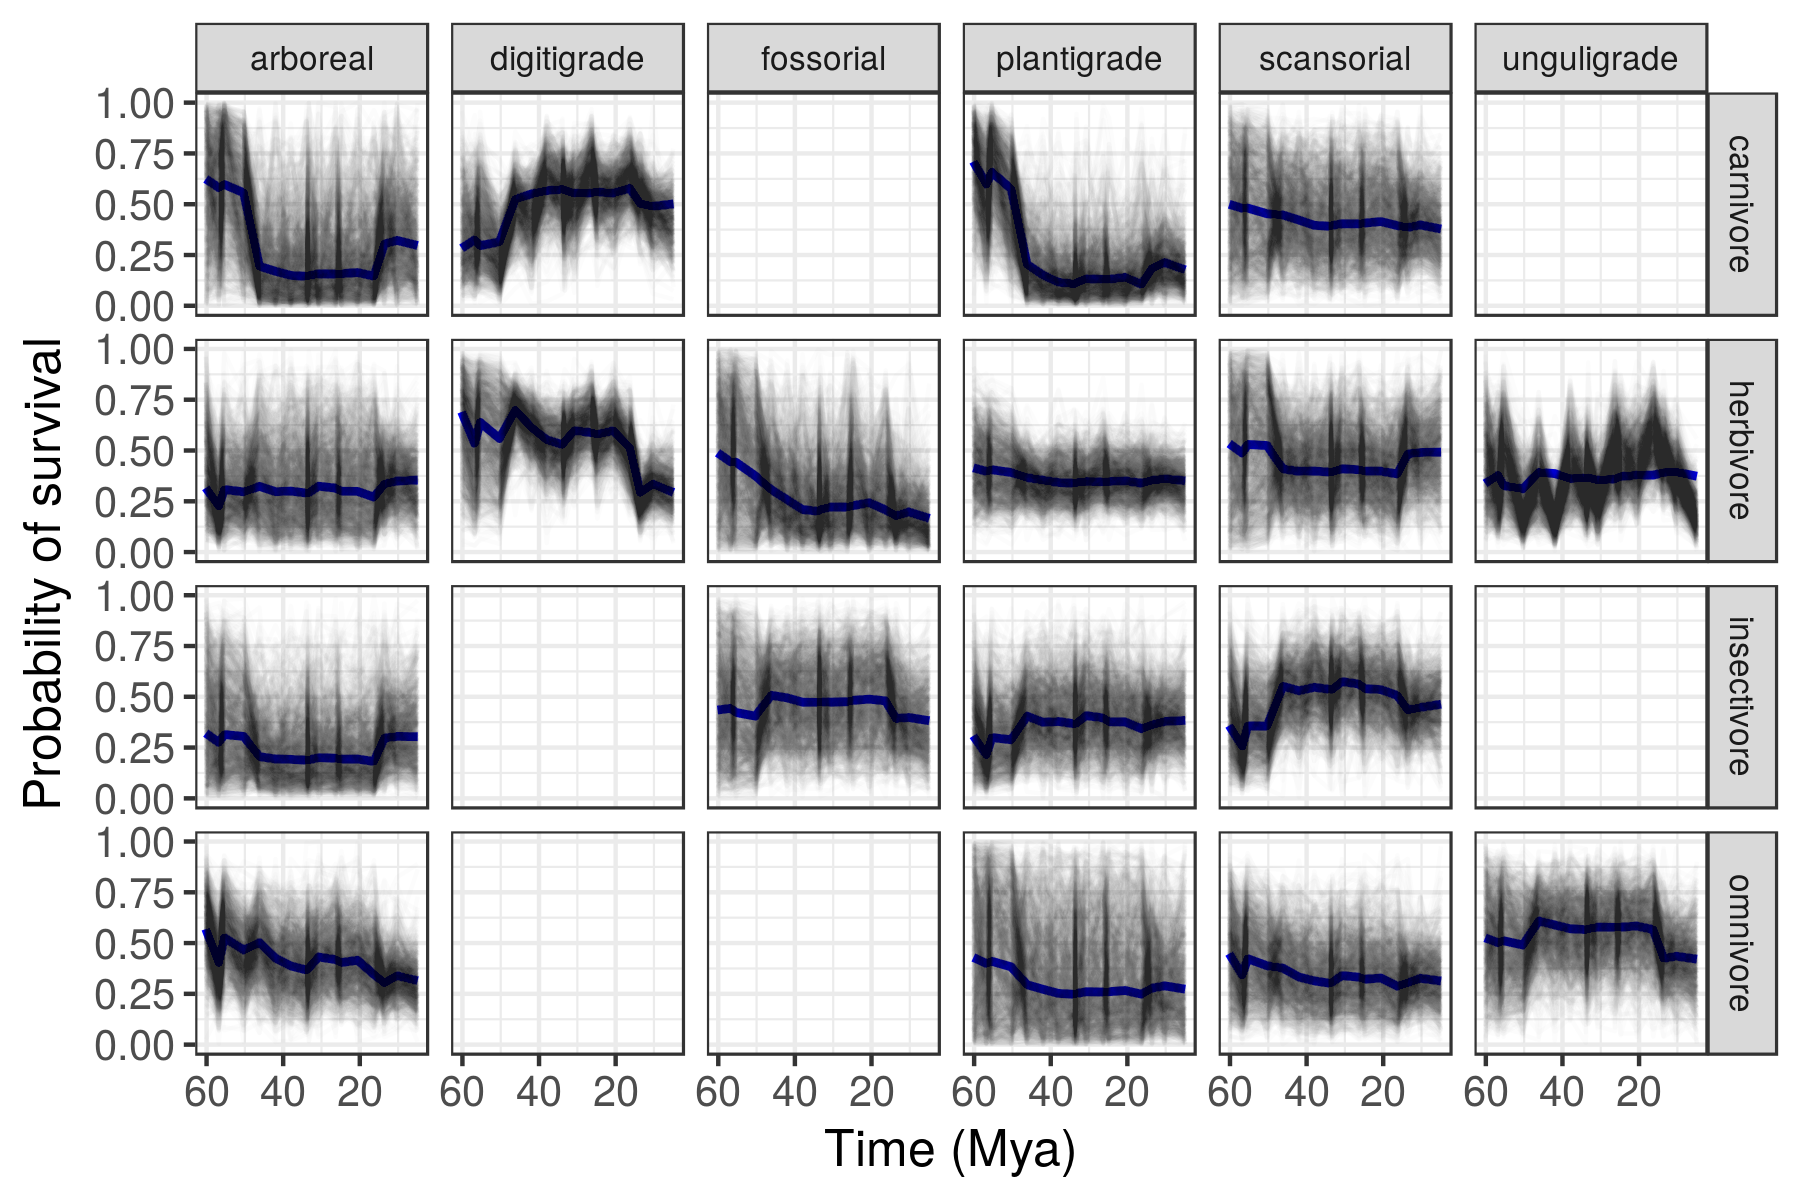
\includegraphics[width=\textwidth,height=0.8\textheight,keepaspectratio=true]{figure/ecotype_survival_bd}
  \caption{Probability of species survival by ecotype. Estimates are from the birth-death model.}
  \label{fig:eco_survival}
\end{figure}

\begin{figure}[ht]
  \centering
  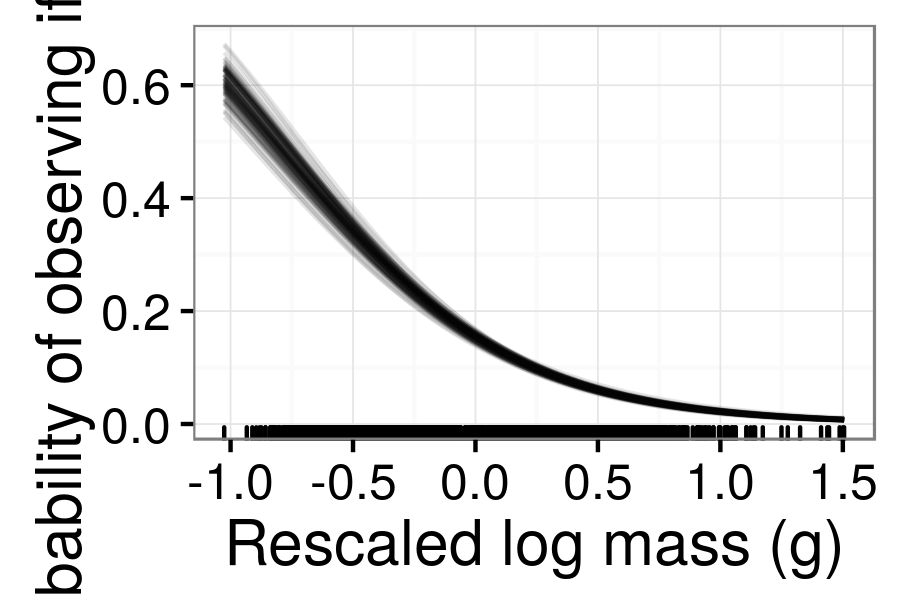
\includegraphics[width=\textwidth,height=0.8\textheight,keepaspectratio=true]{figure/mass_on_samp}
  \caption{Effect of mass on probability of species preservation. Estimates are from the pure-presence model.}
  \label{fig:mass_preserve_pure_pres}
\end{figure}

\begin{figure}[ht]
  \centering
  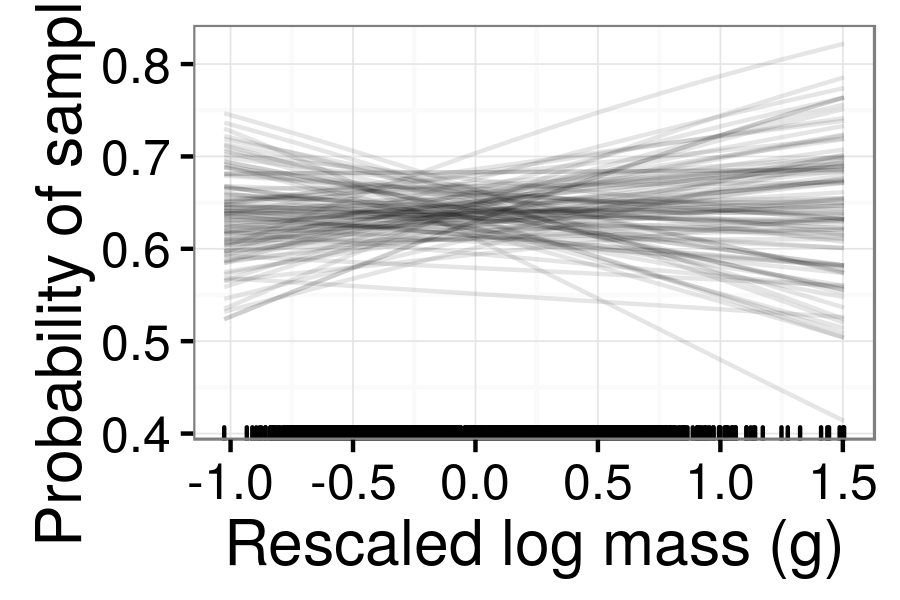
\includegraphics[width=\textwidth,height=0.8\textheight,keepaspectratio=true]{figure/mass_on_samp_bd}
  \caption{Effect of mass on probability of species preservation. Estimates are from the birth-death model.}
  \label{fig:mass_preserve_bd}
\end{figure}

\begin{figure}[ht]
  \centering
  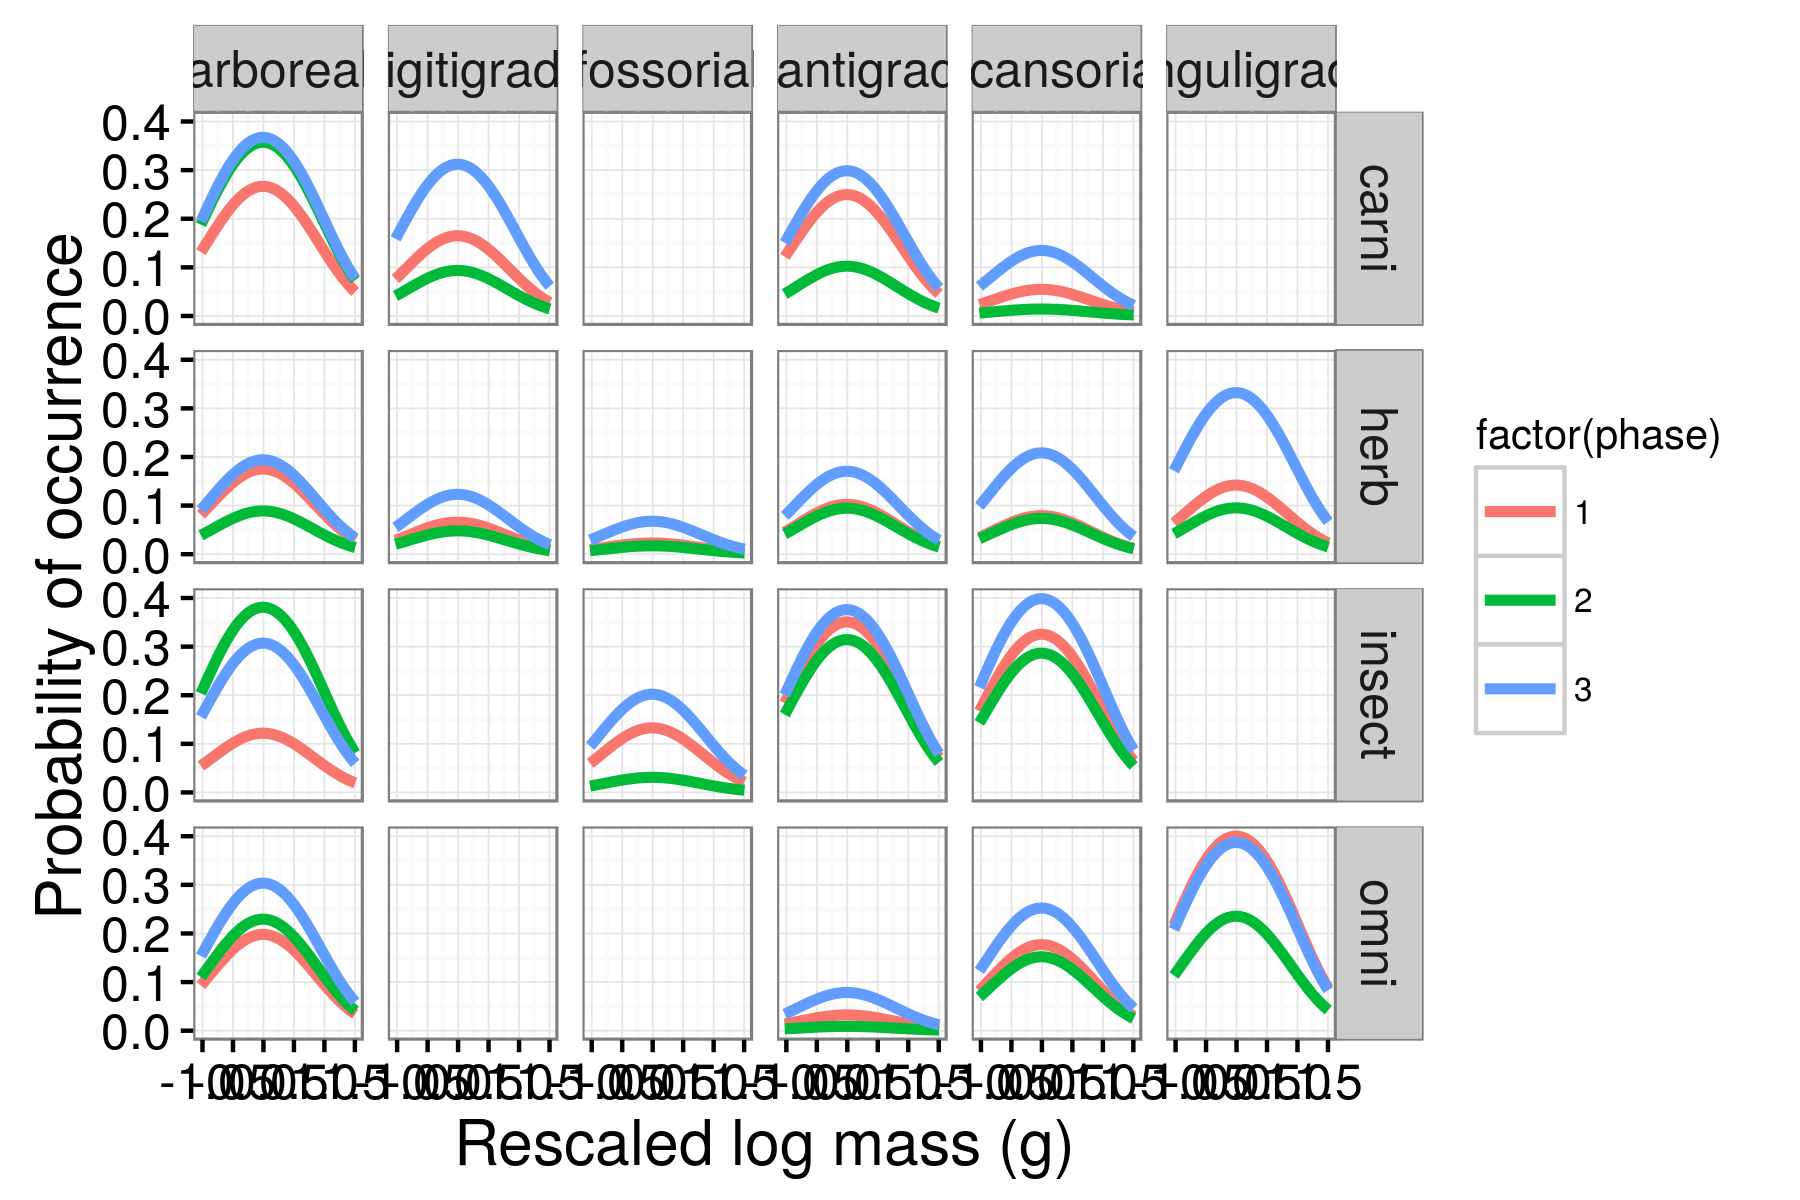
\includegraphics[width=\textwidth,height=0.8\textheight,keepaspectratio=true]{figure/mass_on_pres}
  \caption{Effect of mass on probability of species occurrence. Estimates are from the pure-presence model.}
  \label{fig:mass_occur}
\end{figure}

\begin{figure}[ht]
  \centering
  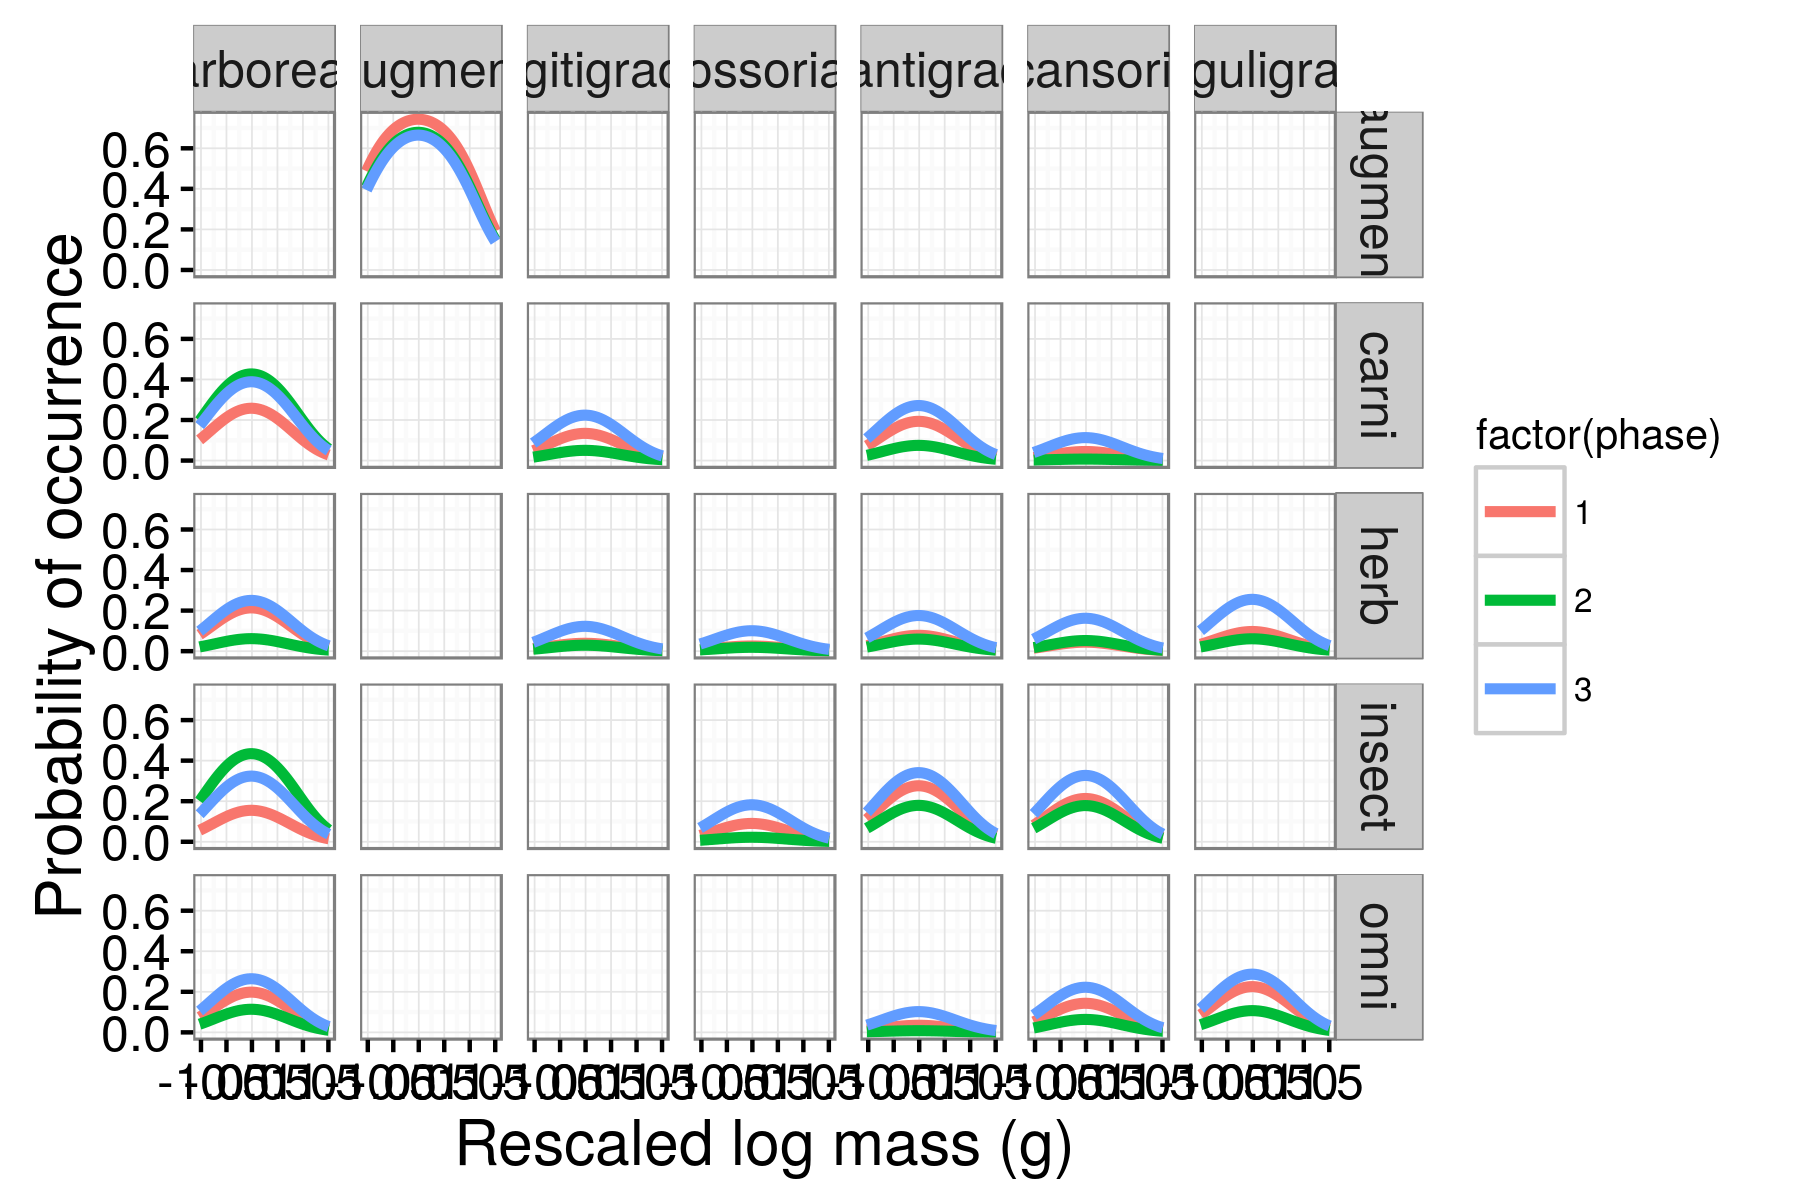
\includegraphics[width=\textwidth,height=0.8\textheight,keepaspectratio=true]{figure/mass_on_origin_bd}
  \caption{Effect of mass on probability of species origination. Estimates are from the birth-death model.}
  \label{fig:mass_origin}
\end{figure}

\begin{figure}[ht]
  \centering
  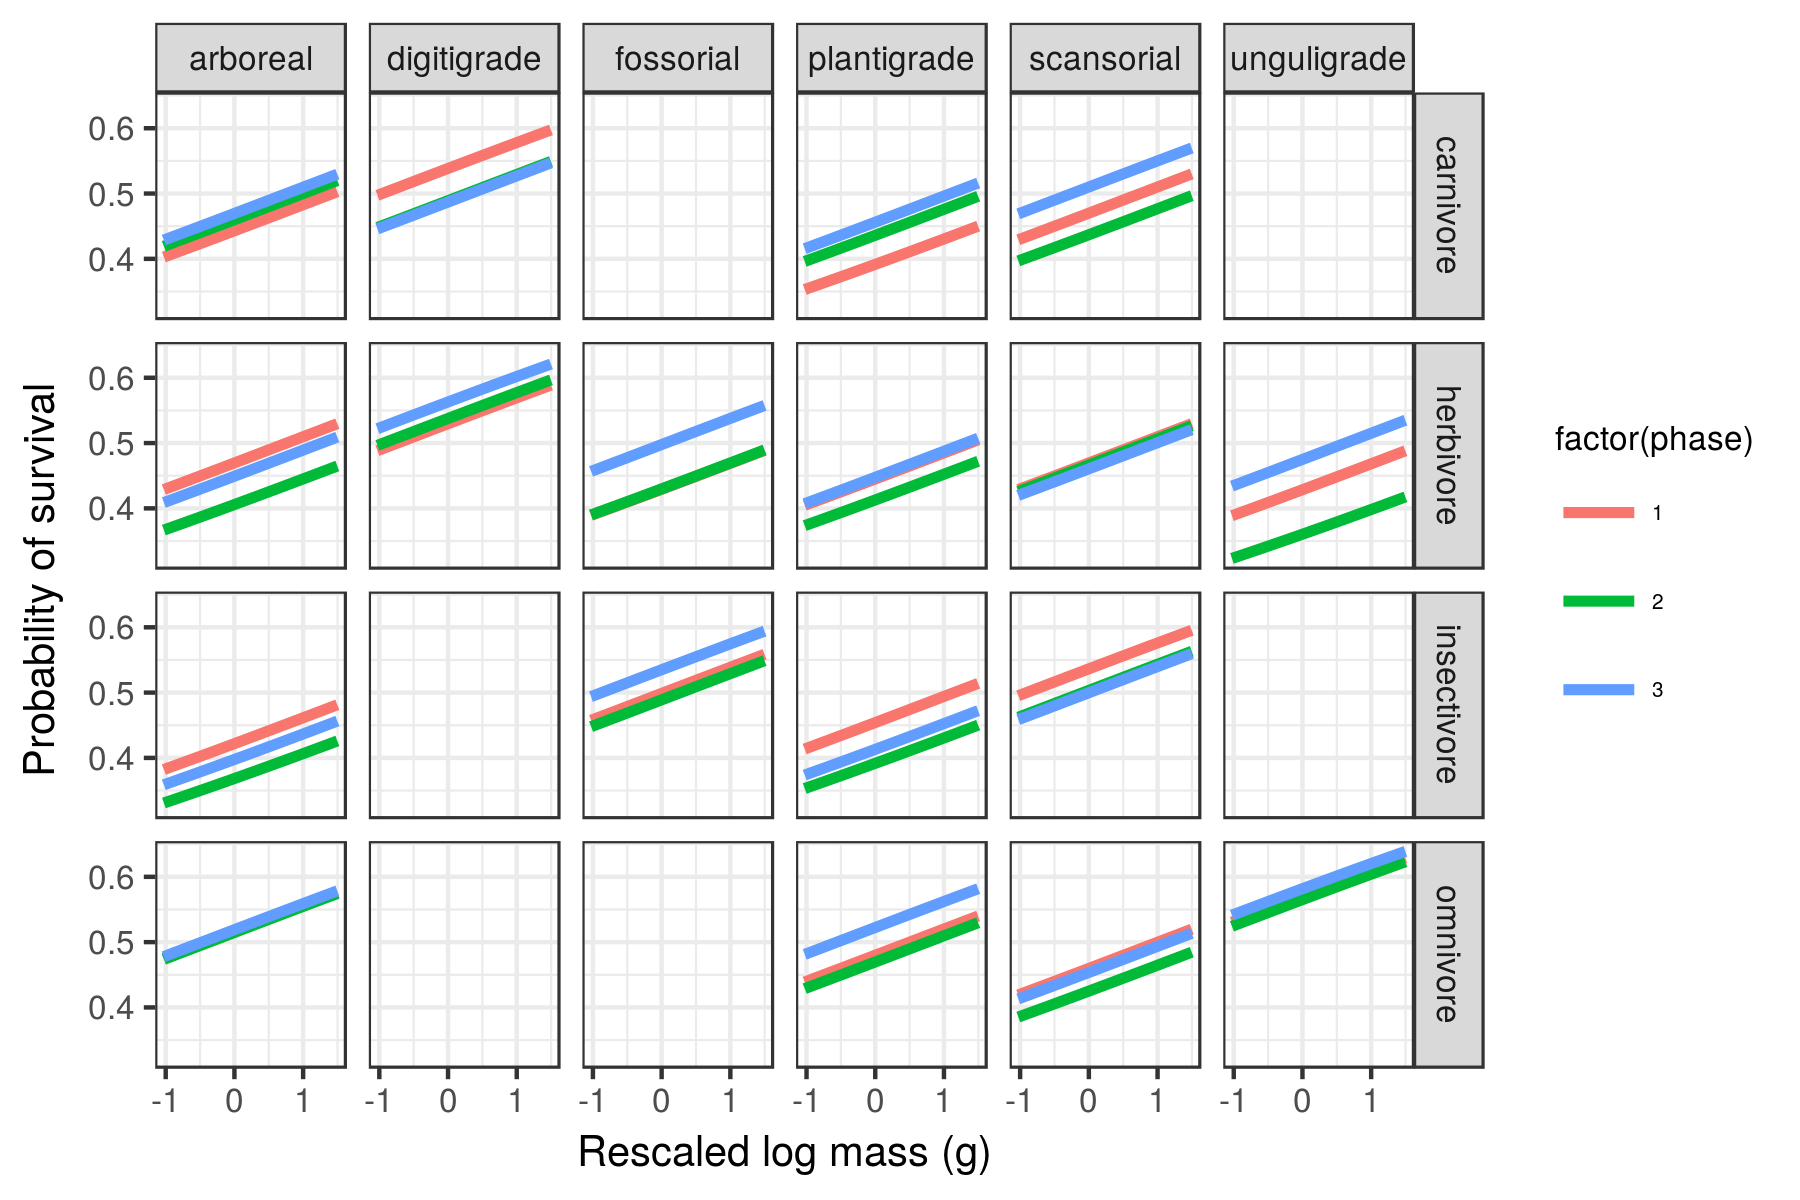
\includegraphics[width=\textwidth,height=0.8\textheight,keepaspectratio=true]{figure/mass_on_surv_bd}
  \caption{Effect of mass on probability of species survival. Estimates are from the birth-death model.}
  \label{fig:mass_survival}
\end{figure}

\begin{figure}[ht]
  \centering
  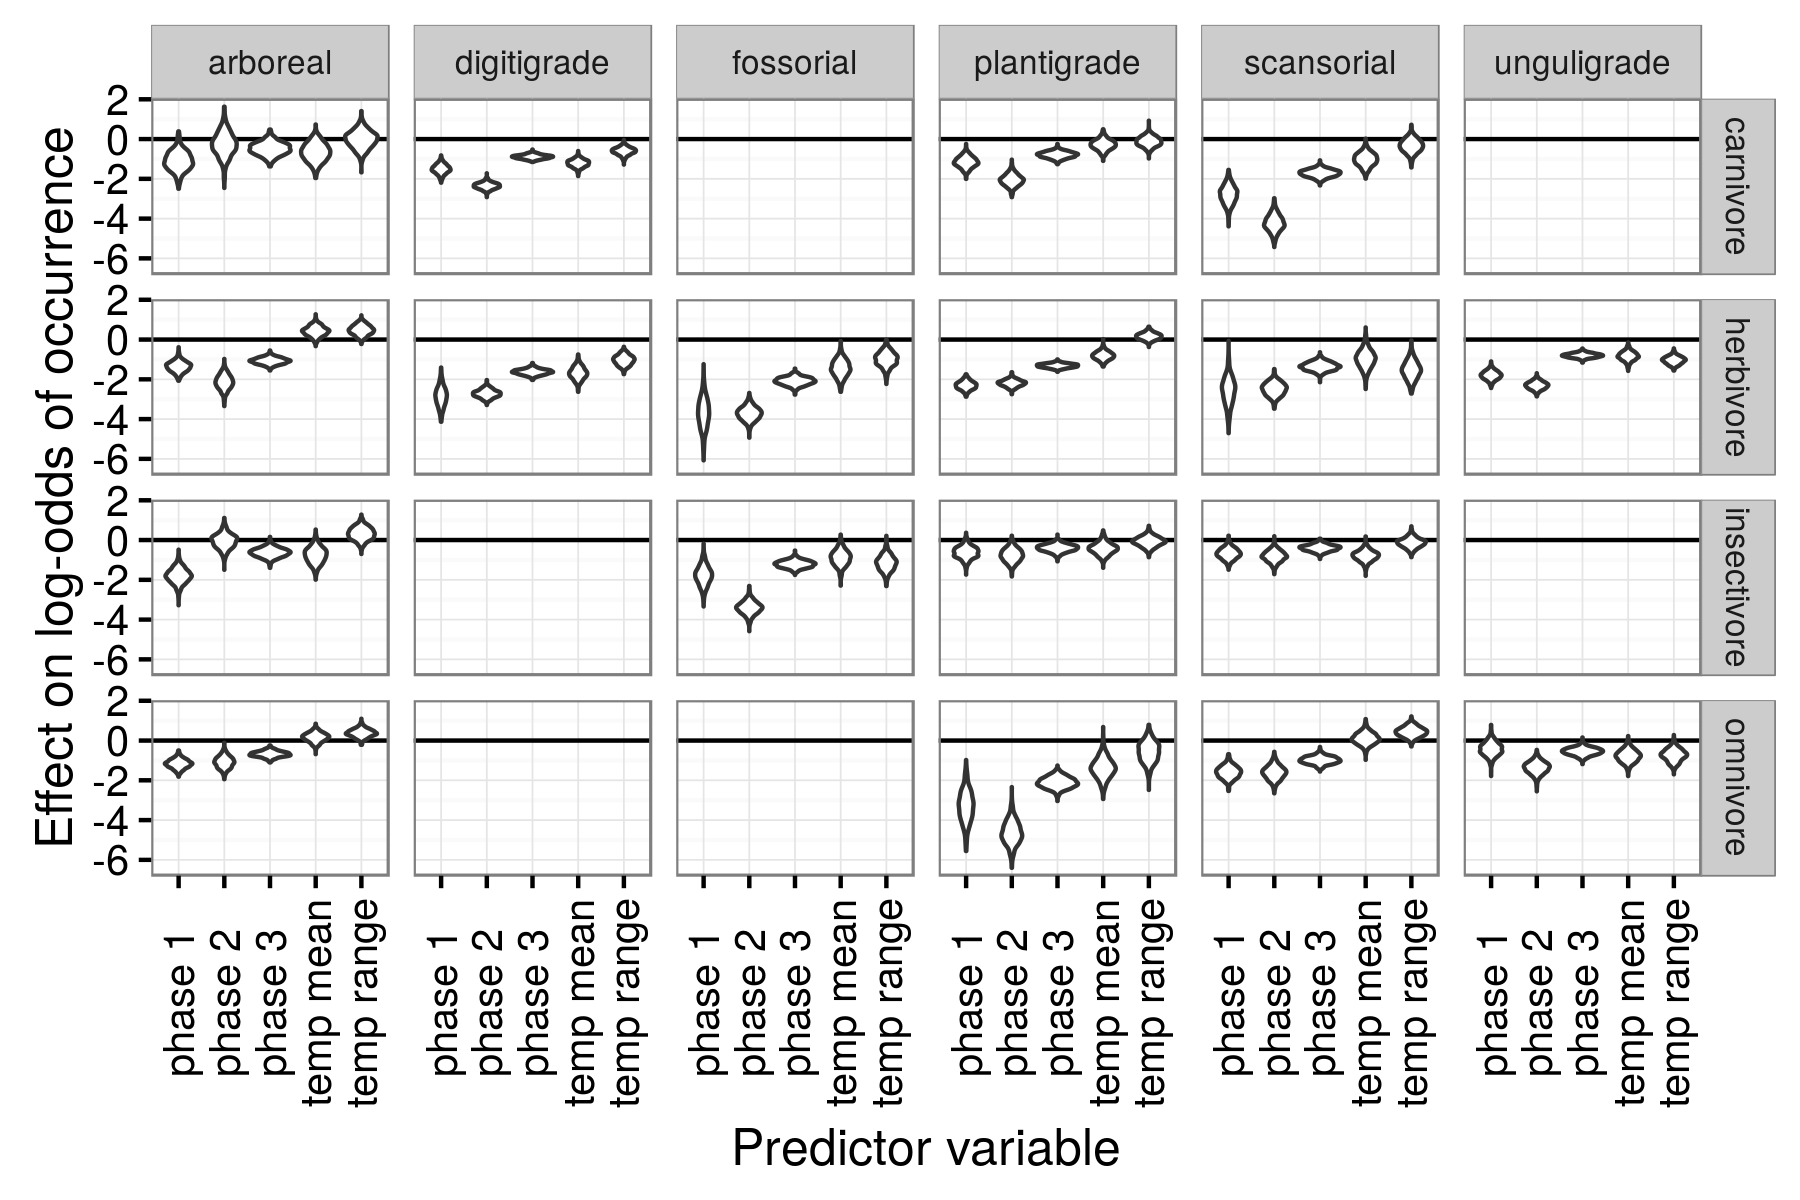
\includegraphics[width=\textwidth,height=0.8\textheight,keepaspectratio=true]{figure/group_on_ecotype}
  \caption{Effects of group-level covariates on log-odds of ecotype occurrence. Estimates are from the pure-presence model.}
  \label{fig:group_pure_presence}
\end{figure}

\begin{figure}[ht]
  \centering
  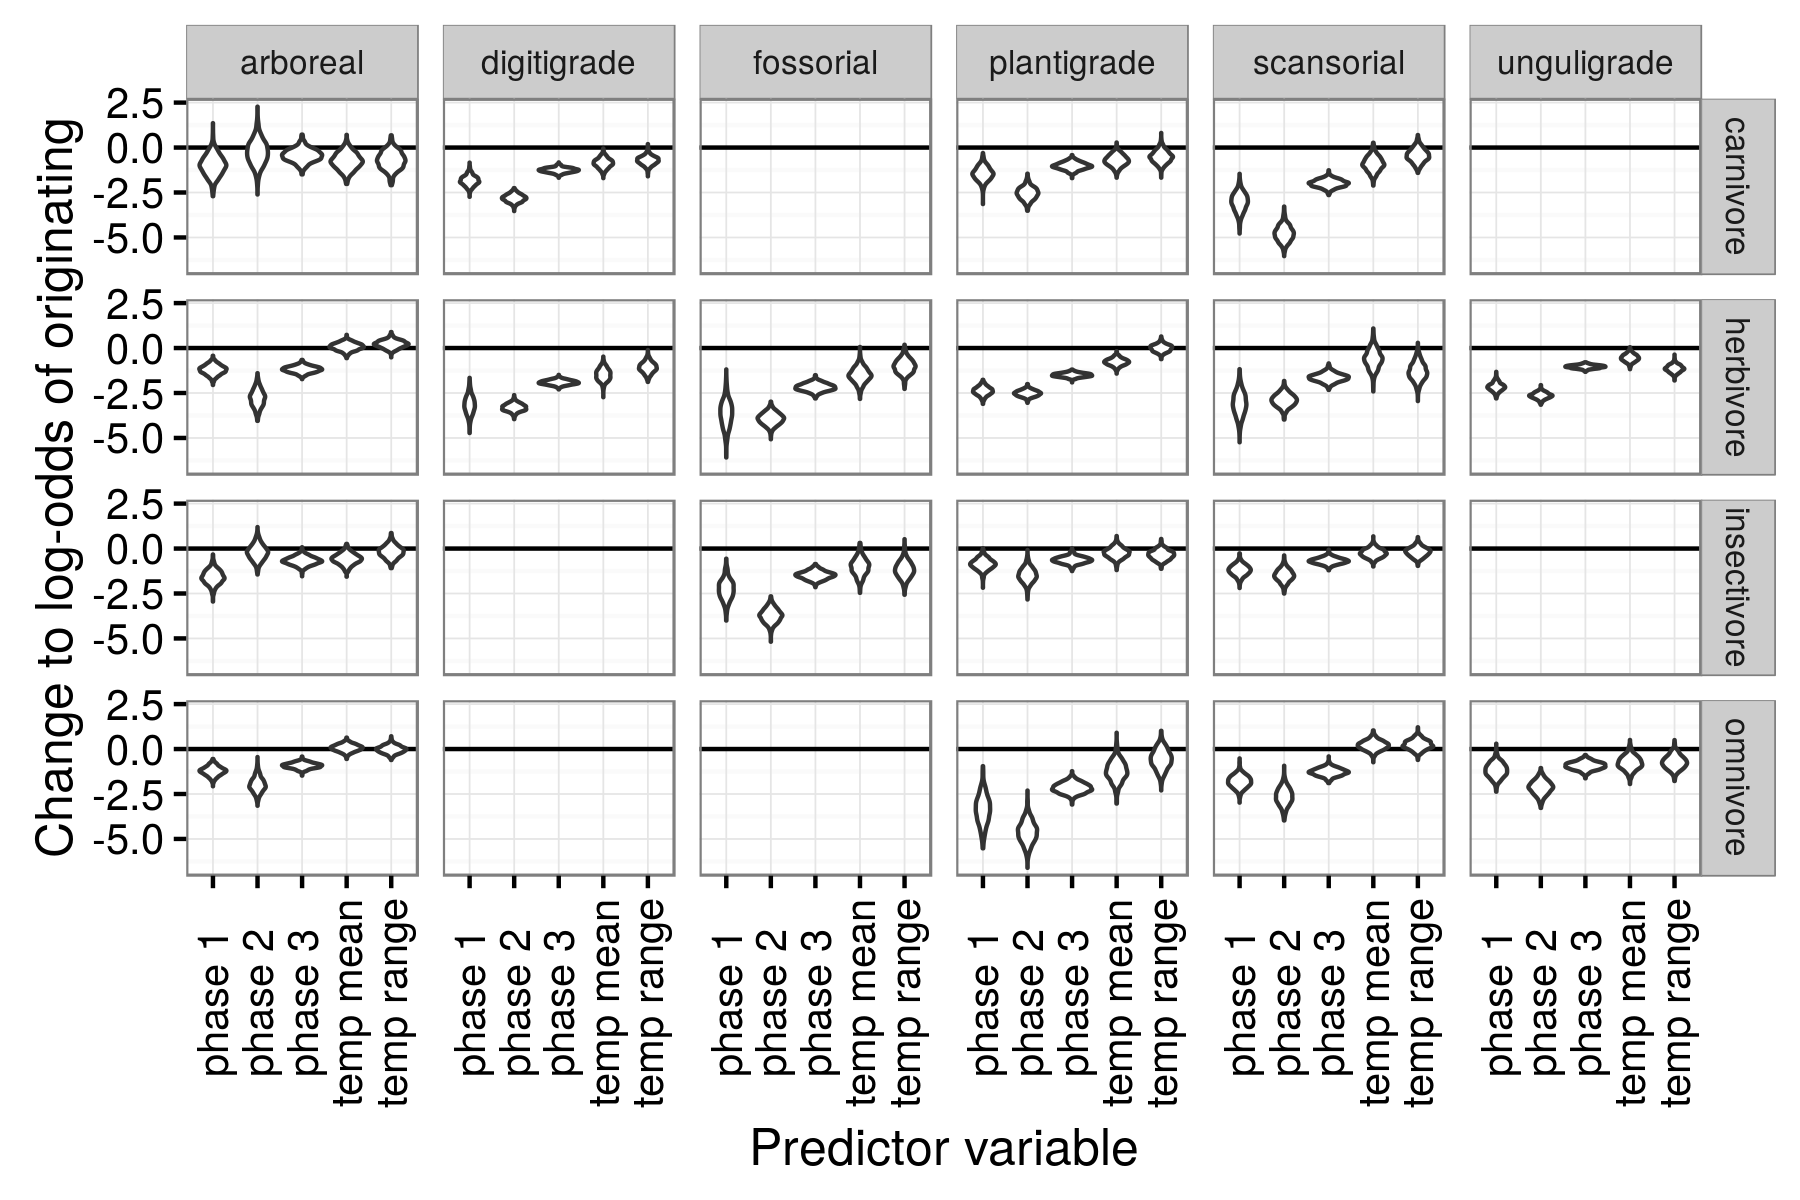
\includegraphics[width=\textwidth,height=0.8\textheight,keepaspectratio=true]{figure/group_on_origin_bd}
  \caption{Effects of group-level covariates on log-odds of origination of species of ecotype. Estimates are from the birth-death model.}
  \label{fig:group_origin_bd}
\end{figure}

\begin{figure}[ht]
  \centering
  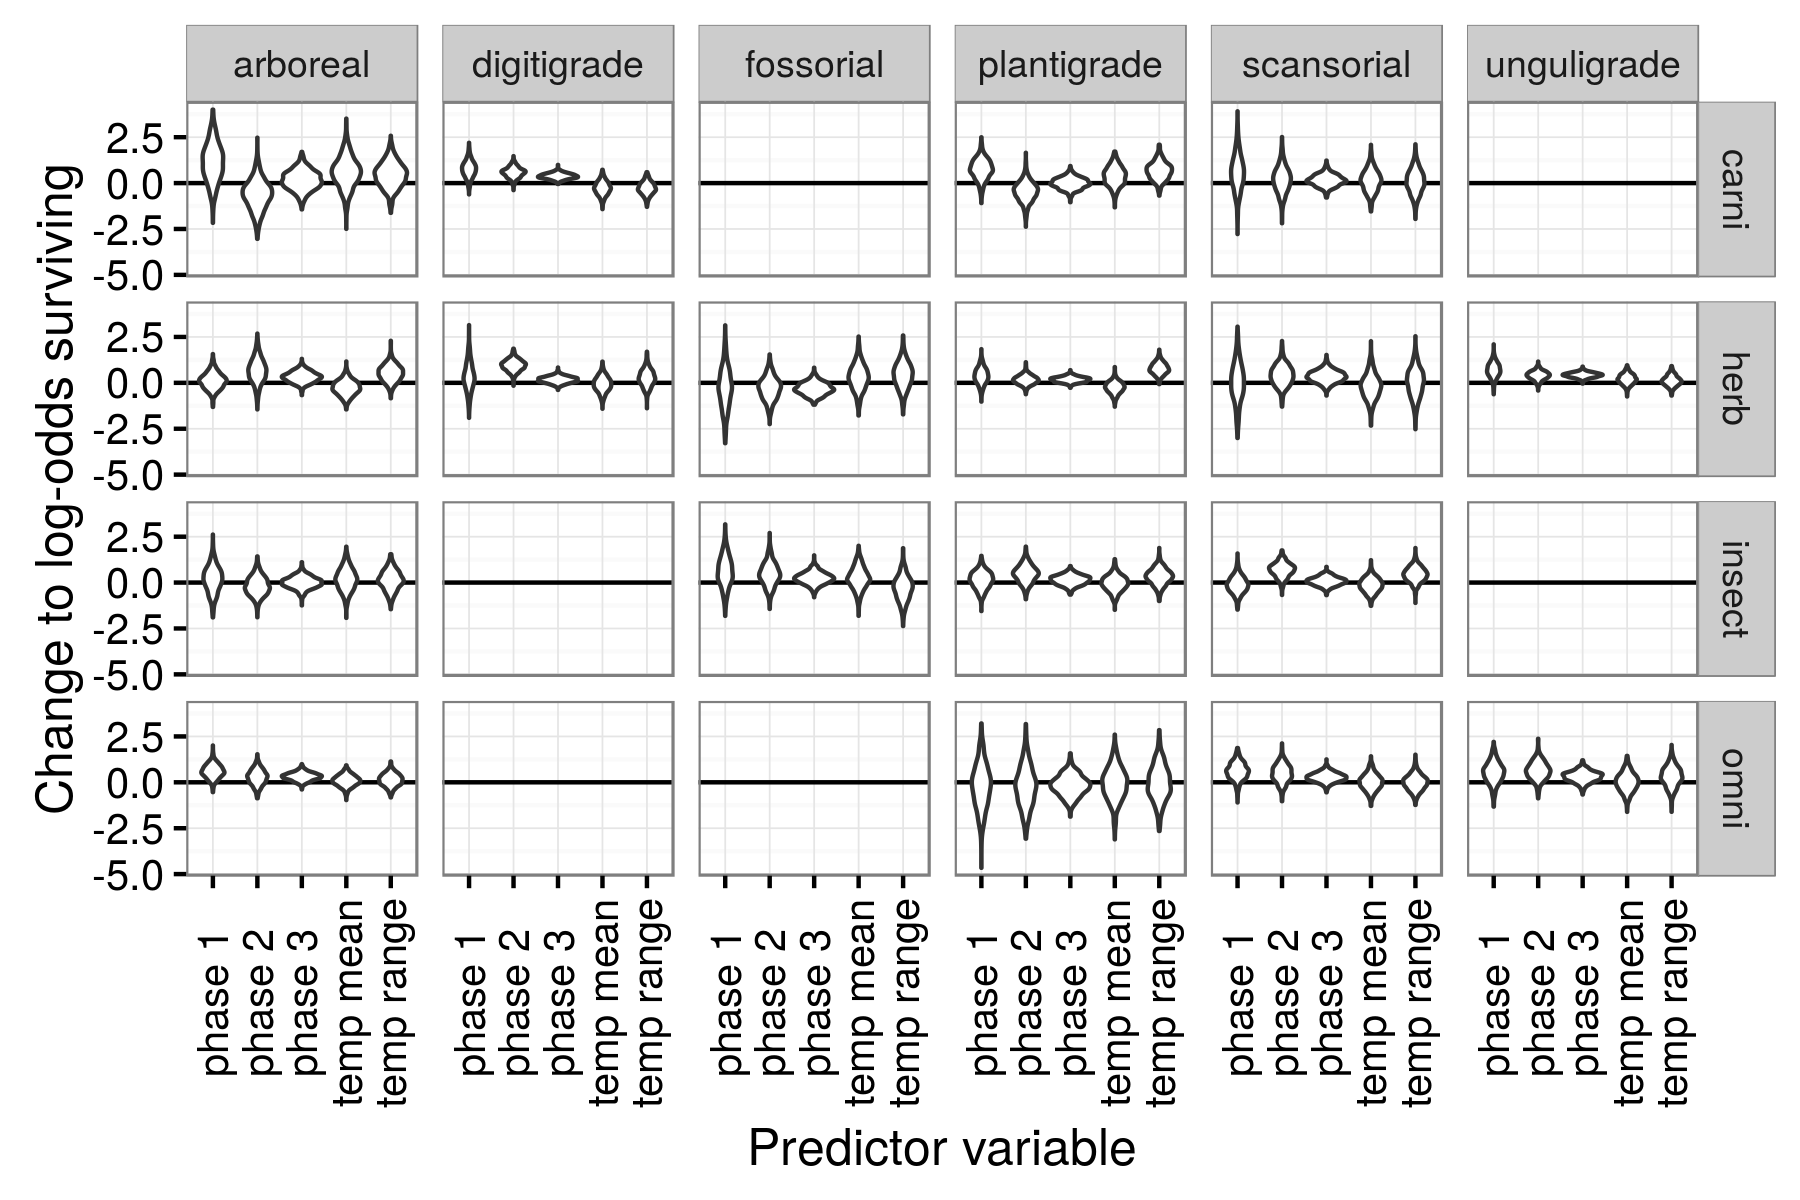
\includegraphics[width=\textwidth,height=0.8\textheight,keepaspectratio=true]{figure/group_on_survival_bd}
  \caption{Effects of group-level covariates on log-odds of survival of species of ecotype. Estimates are from the birth-death model.}
  \label{fig:group_surv_bd}
\end{figure}





\subsection*{Analysis of diversity}


\end{document}
